\documentclass[11pt, letterpaper]{article}
\usepackage[utf8]{inputenc}
\usepackage[letterpaper, margin=0.5in]{geometry}
\usepackage{amsmath}
\usepackage{amssymb}
\usepackage{amsthm}
\usepackage{graphicx}
\usepackage{listings}
\usepackage[font=scriptsize]{caption}
\usepackage{subcaption}
\usepackage{xcolor}

\definecolor{codegreen}{rgb}{0,0.6,0}
\definecolor{codegray}{rgb}{0.5,0.5,0.5}
\definecolor{codepurple}{rgb}{0.58,0,0.82}
\definecolor{backcolour}{rgb}{0.95,0.95,0.92}

\lstdefinestyle{mystyle}{
    backgroundcolor=\color{backcolour},   
    commentstyle=\color{codegreen},
    keywordstyle=\color{magenta},
    numberstyle=\tiny\color{codegray},
    stringstyle=\color{codepurple},
    basicstyle=\ttfamily\footnotesize,
    breakatwhitespace=false,
    texcl=true,
    mathescape=true,
    breaklines=true,                 
    captionpos=b,                    
    keepspaces=true,                 
    numbers=left,                    
    numbersep=5pt,                  
    showspaces=false,                
    showstringspaces=false,
    showtabs=false,                  
    tabsize=2
}

\lstset{style=mystyle}
\graphicspath{ {.} }
\captionsetup{justification=raggedright, singlelinecheck=false}

\author{Ryan Tang}
\title{STA 602 HW 10}
\date{November 11th 2022}

\begin{document}
\maketitle

\section{Exercise 7.4}
\paragraph{(a)}
Here I decided to use a prior that doesn't content much of information with a sprinkle of my guesses.
\begin{align*}
    \theta &\thicksim \mathcal{N}(\theta|
        \mu_0=\begin{bmatrix}35\\33\end{bmatrix},
        \Sigma_0=\begin{bmatrix}5,0\\0,5\end{bmatrix}
    ) \\
    \Sigma &\thicksim IW(\Sigma|\nu_o = 3, S_o =\begin{bmatrix}100,60\\60,100\end{bmatrix})
\end{align*}

Below are 3 draws of prior predictive distribution samples resulted from the above prior specifications.
\begin{figure*}[!h]
  \centering
  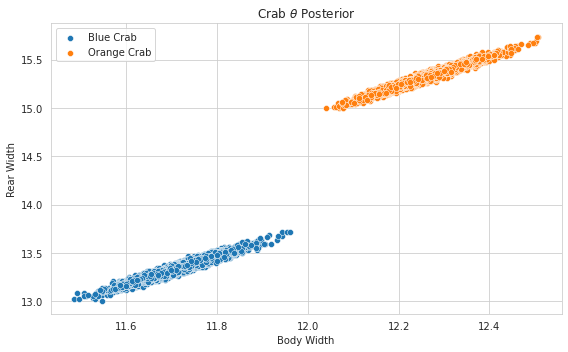
\includegraphics[width=0.5\textwidth]{3.1.png}
  \captionsetup{justification=centering}
  \caption{$\theta$ Posteriors Comparison of two Crabs}
\end{figure*}


\section{Exercise 7.5}
\section{Exercise 7.6}


\end{document}